% Figure: the reasoning boundary (story 4).
% Build: pdflatex reasoning_boundary.tex  (run inside figures/)
\documentclass[tikz,border=6pt]{standalone}
\usetikzlibrary{positioning,arrows.meta,fit,backgrounds}
\begin{document}
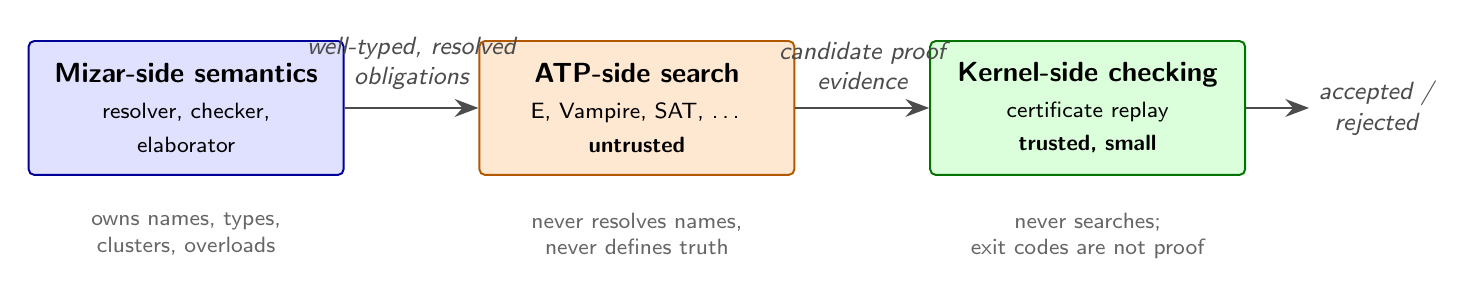
\begin{tikzpicture}[
  font=\sffamily,
  stage/.style={draw, rounded corners=2pt, align=center, minimum width=40mm,
                minimum height=17mm, line width=0.7pt, inner sep=2.5mm},
  artifact/.style={font=\sffamily\small\itshape, align=center, text=black!70},
  rule/.style={font=\sffamily\footnotesize, align=center, text=black!60},
  flow/.style={-{Stealth[length=3mm]}, line width=1pt, black!70},
  node distance=6mm and 17mm,
]
  \node[stage, fill=blue!12, draw=blue!60!black]
    (sem) {\textbf{Mizar-side semantics}\\[1pt]
           \footnotesize resolver, checker,\\ \footnotesize elaborator};
  \node[stage, fill=orange!18, draw=orange!70!black, right=of sem]
    (atp) {\textbf{ATP-side search}\\[1pt]
           \footnotesize E, Vampire, SAT, \dots\\ \footnotesize\bfseries untrusted};
  \node[stage, fill=green!14, draw=green!45!black, right=of atp]
    (ker) {\textbf{Kernel-side checking}\\[1pt]
           \footnotesize certificate replay\\ \footnotesize\bfseries trusted, small};

  \draw[flow] (sem) -- node[artifact, above=1mm, midway] {well-typed, resolved\\ obligations} (atp);
  \draw[flow] (atp) -- node[artifact, above=1mm, midway] {candidate proof\\ evidence} (ker);

  \node[rule, below=3.5mm of sem] {owns names, types,\\ clusters, overloads};
  \node[rule, below=3.5mm of atp] {never resolves names,\\ never defines truth};
  \node[rule, below=3.5mm of ker] {never searches;\\ exit codes are not proof};

  \node[artifact, right=8mm of ker, align=center]
    (out) {accepted /\\ rejected};
  \draw[flow] (ker) -- (out);
\end{tikzpicture}
\end{document}
